\documentclass{amsart}

\usepackage{graphicx}
\usepackage{textcomp}
\usepackage{amsmath}
\usepackage{amsthm}

\newtheorem{theorem}{Theorem}[section]

\renewcommand{\vec}{\textbf}

\theoremstyle{definition}
\newtheorem{definition}{Definition}

\title{Projectile Motion on a Space Station}

\begin{document}
\begin{abstract}
 Something
\end{abstract}
\maketitle


\section{Gravity via centripetal acceleration}


In science fiction, artificial gravity for space-craft and
space-stations is often generated via centripetal acceleration, see
\cite{2001,2010,missiontomars,themartian,expanse,babylon5,europareport,ringworld?,rama,intersetller,etc}
for an incomplete list. Usually characters live inside a cylinder that
is spinning, such as the von Braun Wheel depicted in figure
\ref{fig:Braun Wheel}.

\begin{figure}[h]
  \centering
  \includegraphics[width=0.5\textwidth]{Von_Braun_1952_Space_Station.jpg}
  %wikipedia von Braun Wheel
  \caption{von Braun Wheel}
  \label{fig:Braun Wheel}
\end{figure}

Centripetal acceleration pushes them against the outside wall of the
cylinder. In television and film, (surely due to production
limitations) this ``artificial gravity'' is portrayed as being an
excellent facsimile for Earth's gravity. In this paper we seek to
answer the question of how accurately centripetal acceleration mimics
gravitational acceleration.


% Papers that did similar things to ours
% http://davidkann.blogspot.com/2014/06/oneill-cylinder-simulator-projectile.html (Build a simulator)
% https://kaiserscience.wordpress.com/physics/rotational-motion/artificial-gravity-in-a-space-station/



While centripetal acceleration (on cylindrical space-craft etc.) has
been extensively studied \cite{papers,anotherpaper}, most of these
studies focus on the fictitious forces present on a space stateion and
the basic consiquences these have on the equations for projectile
motion. In this paper we seek to expand on these papers and flush out projectile motion on
spaceship with centripital acceleration. Ultimately we should become
comfortable with projectile motion and we should provide some basic
answers to questions like: What is the maximum height of a projectile?
At what point does a projectile ``loop'' around? How might one play a
game of catch on a ship with centripital acceleration?

\subsection{Projectile Motion from Ring World Inhabitant Perspective}


When on a planet where the acceleration due to gravity is $g$, we know
that an object thrown at an angle of $\theta$ from the horizontal at
an initial speed of $v_0$, with an initial position of $(x_0,y_0)$
follows the path of:
\begin{align*}
  x_{\mathrm{planet}}(t) &=  v_0 t \cos(\theta)  + x_0\\
  y_{\mathrm{planet}}(t) &=  -g/2 t^2 + v_0 t \sin(\theta)  + y_0
\end{align*}
These equations of projectile motion describe the path an object takes
after being thrown.

%Generic gravity Projectile motion plot
\begin{figure}[h]
  \centering
  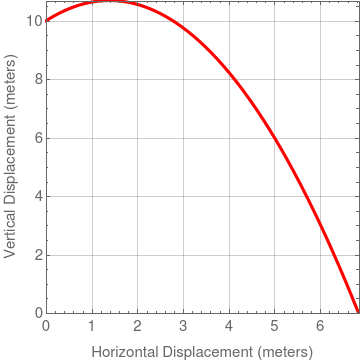
\includegraphics[width=0.5\textwidth]{Projectile_In_Gravity.png}
  \caption{Projectile thrown in standard gravity takes the path of a parabola.}
  \label{fig:Braun Wheel}
\end{figure}

We seek analogous equations that show the path of a projectile on a
rotating space station. In particular, we wish to show the path from
the view-point of people on the station.  From this perspective,
\textit{vertical} is defined as the distance from the floor of the
habitation ring and \textit{horizontal} is defined as the arc length
counter clockwise or clockwise from the observer.

[[image]]


Thus the equations of motion for a projectile ((seems a bit quick!))
from the Ring World Inhabitant Perspective are:

\begin{align*}
  p_{r}(t) &= t^2 (v_x + \omega r_0 \cos(\omega t_0))^2 + (t(v_y + \omega
  r_0 \sin(\omega t_0) - R))^2\\
  p_{\theta R}(t) &=R \arctan(t(V_x + \omega r_0 \cos(\omega t_0)),tV_y +
                    t \omega r_0 \sin(\omega t_0))
\end{align*}

\begin{figure}[h]
  \centering
  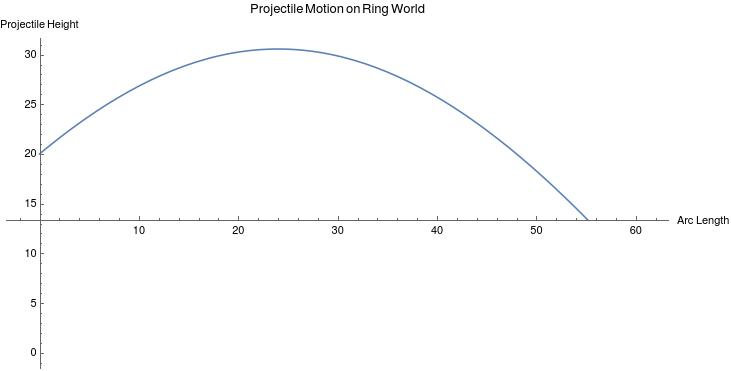
\includegraphics[width=0.7\textwidth]{ArclengthProjectileLabeled.jpg}
  \label{fig:shipview}
  \caption{}
\end{figure}


\begin{figure}[h]
  \centering
  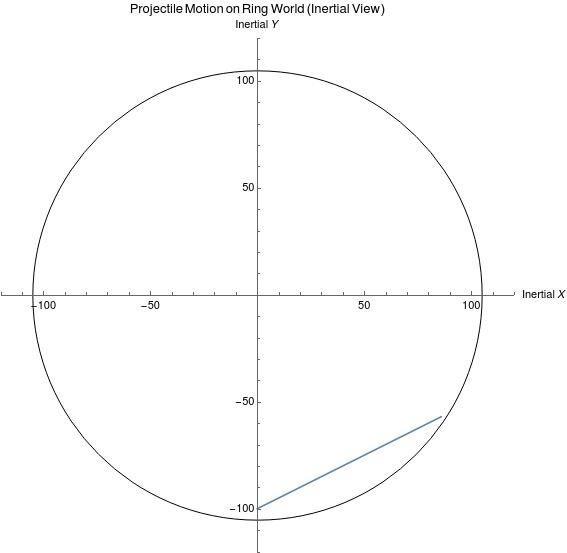
\includegraphics[width=0.7\textwidth]{InertialArclengthProjectileLabeled.jpg}
  \label{fig:inertialview}
  \caption{}
\end{figure}

Figure \ref{fig:shipview} depicts projectile motion (a ball thrown at
45 degrees) using the Ring World equations of motion above. Note that
figure \ref{fig:inertialview} depicts the same throw event in figure
\ref{fig:inertialview}, except from the outside inertial
perspective. Something interesting to note is that from the outside
perspective,the ball is not being thrown at a 45 degree angle with
respect to the thrower's horizontal axis (I wonder why that is).


\section{Acrobatics}



\begin{theorem}
  Given a space station of radius $r$ and angluar velocity $\omega$, the maximum height that can be thrown with realistic behavior is....
\end{theorem}

\begin{theorem}
  How many loops
\end{theorem}


\begin{theorem}
  How many loops
\end{theorem}


\end{document}



